
%%
%% forked from https://gits-15.sys.kth.se/giampi/kthlatex kthlatex-0.2rc4 on 2020-02-13
%% expanded upon by Gerald Q. Maguire Jr.
%% This template has been adapted by Anders Sjögren to the University
%% Engineering Program in Computer Science at KTH ICT. Adaptation is the
%% translation of English headings into Swedish as the addition of Swedish
%% text. Original body text is deliberately left in English.


%% set the default lanage to english or swedish by passing an option to the documentclass - this handles the inside tile page
\documentclass[english]{kththesis}
%\documentclass[swedish]{kththesis}

% \usepackage[style=numeric,sorting=none,backend=biber]{biblatex}

\setlength {\marginparwidth }{2cm} %leave some extra space for todo notes
\usepackage{todonotes}

\usepackage[perpage,para,symbol]{footmisc} %% use symbols to ``number'' footnotes and reset which symbol is used first on each page

\usepackage{comment}
\usepackage{minted}
\usepackage{listings}
\usepackage{color}

\definecolor{dkgreen}{rgb}{0,0.6,0}
\definecolor{gray}{rgb}{0.5,0.5,0.5}
\definecolor{mauve}{rgb}{0.58,0,0.82}

\lstset{frame=tb,
  language=Java,
  aboveskip=3mm,
  belowskip=3mm,
  showstringspaces=false,
  columns=flexible,
  basicstyle={\small\ttfamily},
  numbers=none,
  numberstyle=\tiny\color{gray},
  keywordstyle=\color{blue},
  commentstyle=\color{dkgreen},
  stringstyle=\color{mauve},
  breaklines=true,
  breakatwhitespace=true,
  tabsize=3
}

%% Reduce hyphenation as much as possible
\hyphenpenalty=15000 
\tolerance=1000
% include a variety of packages that are useful

%%----------------------------------------------------------------------------
%%   pcap2tex stuff
%%----------------------------------------------------------------------------
%\usepackage[dvipsnames*,svgnames]{xcolor} %% For extended colors
\usepackage{tikz}
\usetikzlibrary{arrows,decorations.pathmorphing,backgrounds,fit,positioning,calc,shapes}
\usepackage{pgfmath}	% --math engine

%% some additional useful packages
\usepackage{rotating}		%% For text rotating
\usepackage{array}		%% For table wrapping
\usepackage{graphicx}	        %% Support for images
\usepackage{float}		%% Suppor for more flexible floating box positioning
\usepackage{mdwlist}            %% various list-related commands
\usepackage{setspace}           %% For fine-grained control over line spacing
\usepackage{listings}		%% For source code listing
\usepackage{bytefield}          %% For packet drawings
\usepackage{tabularx}		%% For simple table stretching
\usepackage{multirow}	        %% Support for multirow colums in tables

\usepackage{url}                %% Support for breaking URLs
\usepackage{hyperref}
\usepackage[all]{hypcap}	%% prevents an issue related to hyperref and caption linking
%% setup hyperref to use the darkblue color on links
\hypersetup{colorlinks,breaklinks,
            linkcolor=darkblue,urlcolor=darkblue,
            anchorcolor=darkblue,citecolor=darkblue}


%% Some definitions of used colors
\definecolor{darkblue}{rgb}{0.0,0.0,0.3} %% define a color called darkblue
\definecolor{darkred}{rgb}{0.4,0.0,0.0}
\definecolor{red}{rgb}{0.7,0.0,0.0}
\definecolor{lightgrey}{rgb}{0.8,0.8,0.8} 
\definecolor{grey}{rgb}{0.6,0.6,0.6}
\definecolor{darkgrey}{rgb}{0.4,0.4,0.4}
\definecolor{aqua}{rgb}{0.0, 1.0, 1.0}

%% If you are going to include source code (or code snippets)
\usepackage{listings}
%%\usepackage[cache=false]{minted} %% For source code highlighting
%%\usemintedstyle{borland}

\usepackage{csquotes} % Recommended by biblatex


%% Acronyms
% note that nonumberlist - removes the cross references to the pages where the acronym appears
% note that nomain - does not produce a main gloassay, this only acronyms will be in the glossary
% note that nopostdot - will present there being a period at the end of each entry
\usepackage[acronym, section=section, nonumberlist, nomain, nopostdot]{glossaries}
%\glsdisablehyper
\makeglossaries
%%% Local Variables:
%%% mode: latex
%%% TeX-master: t
%%% End:

\newacronym{DSL}{DSL}{Domain-specific Language}
\newacronym{DSR}{DSR}{Design Science Research}
\newacronym{MAL}{MAL}{Meta Attack Language}
\newacronym{OS}{OS}{Operative System}
                %load the acronyms file

%% definition of new command for bytefield package
\newcommand{\colorbitbox}[3]{%
	\rlap{\bitbox{#2}{\color{#1}\rule{\width}{\height}}}%
	\bitbox{#2}{#3}}

\newenvironment{swedishnotes}%
  {\begin{center}
      \selectlanguage{swedish}
      \color{blue}}%
    {\end{center}\selectlanguage{english}
    }
  
\begin{document}
\ifinswedish
    \selectlanguage{swedish}
\else
\selectlanguage{english}
\fi


%% Information for inside title page
\title{Validating a threat modeling language for enterprise systems}
%\subtitle{An subtitle in the language of the thesis}

% give the alternative title - i.e., if the thesis is in English, then give a Swedish title
\alttitle{Validera ett hotmodelleringsspråk för företagssystem}
%\altsubtitle{Detta är den svenska översättningen av undertiteln}
% alternative, if the thesis is in Swedish, then give an English title
%\alttitle{This is the English translation of the title}
%\altsubtitle{This is the English translation of the subtitle}

\authorsLastname{Yaasin}
\authorsFirstname{Hassan Ali}
\email{yaasin@kth.se}
\kthid{u100001}
% If the student has an ORCiD - add it here
\orcid{0000-0002-00001-1234}
\authorsSchool{\schoolAcronym{EECS}}

\supervisorAsLastname{Masoudi}
\supervisorAsFirstname{Meysam}
\supervisorAsEmail{masoudi@kth.se}
% If the supervisor is from within KTH add their KTHID, School and Department info
\supervisorAsKTHID{u100003}
\supervisorAsSchool{\schoolAcronym{EECS}}
\supervisorAsDepartment{Computer Science}
% other for a supervisor outside of KTH add their organization info
%\supervisorAsOrganization{Timbuktu University, Department of Pseudoscience}

%If there is a second supervisor add them here:
%\supervisorBsLastname{Supervisor}
%\supervisorBsFirstname{Another Busy}
%\supervisorBsEmail{sb@kth.se}
% If the supervisor is from within KTH add their KTHID, School and Department info
%\supervisorBsKTHID{u100003}
%\supervisorBsSchool{\schoolAcronym{ABE}}
%\supervisorBsDepartment{Public Buildings}
% other for a supervisor outside of KTH add their organization info
%\supervisorBsOrganization{Timbuktu University, Department of Pseudoscience}

\examinersLastname{Slimane}
\examinersFirstname{Ben Slimane}
\examinersEmail{slimane@kth.se}
% If the examiner is from within KTH add their KTHID, School and Department info
\examinersKTHID{u100004}
\examinersSchool{\schoolAcronym{EECS}}
\examinersDepartment{Computer Science}
% other for a examiner outside of KTH add their organization info
%\examinersOrganization{Timbuktu University, Department of Pseudoscience}


\hostcompany{MITRE ATT\&CK} % Remove this line if the project was not done at a host company
%\hostorganization{CERN}   % if there was a host organization

\date{\today}

\programcode{TIEDB}
%% Alternatively, you can say \programme{Civilingenjör Datateknik} to directly set the programme string

\titlepage
% document/book information page
\bookinfopage

% Frontmatter includes the abstracts and table-of-contents
\frontmatter
\setcounter{page}{1}
\begin{abstract}
  \markboth{\abstractname}{}
  \begin{comment}
  
  \todo[inline]{The first abstract should be in the language of the thesis.}
  \todo[inline, backgroundcolor=aqua]{Abstract fungerar på svenska också.}

\todo[inline]{Keep in mind that most of your potential readers are only going to read your title and abstract. This is why it is important that the abstract give them enough information that they can decide is this document relevant to them or not. Otherwise the likely default choice is to ignore the rest of your document.\\
A abstract should stand on its own, i.e., no citations, cross references to the body of the document, acronyms must be spelled out, …\\
Write this early and revise as necessary. This will help keep you focused on what you are trying to do.}

Write an abstract\todo{Use about 1/2 A4-page (250 and 350 words).}  with the following components:
\begin{itemize}
  \item What is the topic area? (optional) Introduces the subject area for the project.
  \item Short problem statement
  \item Why was this problem worth a Master’s thesis project? (i.e., why is the problem both significant and of a suitable degree of difficulty for a Master’s thesis project? Why has no one else solved it yet?)
  \item How did you solve the problem? What was your method/insight?
  \item Results/Conclusions/Consequences/Impact: What are your key results/conclusions? What will others do based upon your results? What can be done now that you have finished - that could not be done before your thesis project was completed?\todo[inline]{The presentation of the results should be the main part of the abstract.}
\end{itemize}
\end{comment}

In today’s era, the systems of the enterprises have developed in a huge effect. The systems have changed into more advanced constructions, able to gather more information and take on more tasks. While the structure of the systems are being more complex, more risks are being accumulated. Nowadays there is a lot of valuable data inside corporations that some people want to get hold of and this could cause a lot of damage in the wrong hands, this possible threat could happen in many various ways. This  is why it has been more important to evolve alternative defense mechanisms to counter these potential attacks and avoid deceptions inside enterprises.\\

\noindent Previously, enterpriseLang was proposed as a domain-specific language based on the meta attack language framework. The purpose of this thesis is to validate enterpriseLang  through creating test cases and calculating the overall test coverage.


\ifinswedish
\subsection*{Nyckelord}
5-6 nyckelord\todo{Nyckelord som beskriver innehållet i uppsatsrapporten}
\else
\subsection*{Keywords}
Threat modeling, Attack simulations, Domain-specific language, Meta Attack language and enterpriseLang.
\fi

\end{abstract}
\cleardoublepage

\ifinswedish
    \selectlanguage{english}
\else
    \selectlanguage{swedish}
\fi
  \begin{abstract}
    \markboth{\abstractname}{}
    

\noindent I dagens tid har företagens system utvecklats med en enorm effekt. Systemen har förändrats till mer avancerade konstruktioner, kan samla mer information och ta på sig fler uppgifter. Medan strukturen i systemen blir mer komplex, ackumuleras fler risker. Numera finns det mycket värdefull information i företag som vissa människor vill få tag på och detta kan orsaka mycket skada i fel händer, detta möjliga hot kan hända på många olika sätt. Det är därför det har varit viktigare att utveckla alternativa försvarsmekanismer för att motverka dessa potentiella attacker och undvika bedrägerier inom företag.\\

\noindent Tidigare föreslogs enterpriseLang som ett domänspecifikt språk baserat på meta attack språkramen. Syftet med denna avhandling är att validera enterpriseLang genom att skapa testfall och beräkna den totala testtäckningen.

\subsection*{Nyckelord}
Hotmodellering, Attack-simuleringar, Domänspecifikt språk, Meta Attack-språk och enterpriseLang.


  \end{abstract}

\cleardoublepage


\cleardoublepage
% set to the language of the body of the thesis
\ifinswedish
    \selectlanguage{swedish}
\else
    \selectlanguage{english}
\fi

\begin{comment}
\section*{Acknowledgments }
\markboth{Acknowledgments}{}
\todo[inline]{It is nice to acknowledge the people that have helped you. It is
  also necessary to acknowledge any special permissions that you have gotten –
  for example getting permission from the copyright owner to reproduce a
  figure. In this case you should acknowledge them and this permission here
  and in the figure’s caption. \\
  Note: If you do not have the copyright owner’s permission, then you cannot use any copyrighted figures/tables/… .
}
\todo[inline, backgroundcolor=aqua]{I detta kapitel kan du e v nämna något om
  din bakgrund om det påverkar rapporten på något sätt. Har du t ex inte
  möjlighet att skriva perfekt svenska för att du är nyanländ till landet kan
  det vara på sin plats att nämna detta här. OBS, detta får dock inte vara en
  ursäkt för att lämna in en rapport med undermåligt språk, grammatik och
  stavning (t ex får fel som en automatisk stavningskontroll och
  grammatikkontroll kan upptäcka inte förekomma)\\

En dualism som måste hanteras i hela rapporten och projektet
}

I would like to thank xxxx for having yyyy.\\

\acknowlegmentssignature
\end{comment}
\fancypagestyle{plain}{}
\renewcommand{\chaptermark}[1]{ \markboth{#1}{}} 
\tableofcontents
  \markboth{\contentsname}{}

\cleardoublepage
\listoffigures

\cleardoublepage

\listoftables
\cleardoublepage
\lstlistoflistings
\cleardoublepage
\printglossary[type=\acronymtype, title={List of acronyms and abbreviations}]

\label{pg:lastPageofPreface}
% Mainmatter is where the actual contents of the thesis goes
\mainmatter

\renewcommand{\chaptermark}[1]{\markboth{#1}{}}
\chapter{Introduction}

Unfortunately, in every system there is a weakness. It is almost impossible to build a software system without any vulnerabilities. This is why the tasks in Cybersecurity exist, to protect the IT systems of companies from Cyber attacks. Together with this, the idea of threat modeling and  attack simulations came up. Threat modeling is a method to anticipate possible vulnerabilities and make amendments to the security. Attack simulations contain methods simulating an attack in an enterprise system containing scenarios of different ways where the opponent has succeeded to harm the system. Enterprises could use both of these methodologies to predict coming cyber threats in the future.

\noindent \\In this bachelor thesis, a domain-specific thread modeling language with the name enterpriseLang will be described. This language originates from \gls{MAL} framework. The work of the bachelor thesis will be described together with key concepts such as \gls{MAL}, \gls{DSL}, thread modeling, attack simulations and the enterpriseLang language.


\section{Background}
\label{sec:background}

\noindent Threat modeling is a method for analysing possible attacks or threats and supplying a plan to a secured software system which is the main target of the adversary. In threat modeling the perspective of the adversary is a great role to understand its goals of attacking a vulnerable system. In this way security weak points can be found to and harnessed for the software system to get ameliorated \cite{xiong2021cyber}.\\

\noindent Attack simulations intend to visualize paths through a system in situation where an antagonist has succeeded the goal to destabilize a software system.There are several tools developed that are aimed to create attack graph based simulations. \gls{MAL} renders probabilistic simulations, MulVal associates weaknesses extracted from scans that are vulnerable against adversary's attacks and derives logical attack graphs from there while k-zero Day Safety broadens MulVal to computation of zero-day attack graphs. Besides while assuming an opponent has access to the vulnerable system, NAVIGATOR regards the known vulnerabilities as instantly utilizable. Furthermore, the Topological Vulnerability Analysis (TVA) models security conditions and with the help of a database of exploits, it uses them as links between the security conditions. A tool with the similar method is NetSecuritas that exploits scanner output for generating attack graphs and matching security recommendations \cite{xiong2021cyber}.


\section{Problem}

Many technical systems in enterprises are being targeted by hackers that want to exploit the data of such organizations. The data infrastructures of such enterprises need to get more solid and secure, this is how we come to the following question. How could enterprises avoid being victims for cyber crime activities?

\begin{comment}

\todo[inline, backgroundcolor=aqua]{svensk: Problemdefinition elle Frågeställning\\
Lyft fram det ursprungliga problemet om det finns något och definiera därefter
den ingenjörsmässiga erfarenheten eller/och vetenskapen som kan komma ur
projektet. }

Longer problem statement\\
If possible, end this section with a question as a problem statement.

% Research Question
\subsection{Original problem and definition}
\todo[inline, backgroundcolor=aqua]{Ursprungligt problem och definition}
Some text

\subsection{Scientific and engineering issues}\todo[inline, backgroundcolor=aqua]{Vetenskaplig och ingenjörsmässig frågeställning}
some text
\end{comment}

\section{Purpose}
%\todo[inline, backgroundcolor=aqua]{Syfte}
The purpose of this thesis and degree project is to facilitate enterprises guarding important information against adversary cyber offenses by creating a language that could strengthen the security of the enterprise systems. After the goals of this project are achieved an enterprise should benefit from the threat modeling language by using the tools provided from the language to prepare against cyber attacks to protect against them.

%\todo[inline, backgroundcolor=aqua]{Skilj på syfte och mål! Syfte är att förändra något till det bättre. I examensarbetet finns ofta två aspekter på detta. Dels vill problemägaren (företaget) få sitt problem löst till det bättre men akademin och ingenjörssamfundet vill också få nya erfarenheter och vetskap. Beskriv ett syfte som tillfredställer båda dessa aspekter.\\
%Det finns även ett syfte till som kan vara värt att beakta och det är att du som student skall ta examen och att du måste bevisa, i ditt examensarbete, att du uppfyller examensmålen. Dessa mål sammanfaller med kursmålen för examensarbetskursen. 
%}

\section{Goals}
%\todo[inline, backgroundcolor=aqua]{Mål}
%\todo[inline, backgroundcolor=aqua]{Skilj på syfte och mål. Syftet är att åstakomma en förändring i något. Målen är vad som konkret skall göras för att om möjligt uppnå den önskade förändringen (syfte). }

The goal of this project is to create unit tests based on real world cyber attacks to verify functionalities in enterpriseLang and eventually solve or update the tests within enterpriseLang if some of them do not work. This goal has been divided into following three sub-goals:

\begin{enumerate}
\item Subgoal 1: %\todo[inline, backgroundcolor=aqua]{för att tillfredsställa problemägaren – industrin?}
\\Collect real world cyber attacks on enterprise systems.
\item Subgoal 2: %\todo[inline, backgroundcolor=aqua]{för att tillfredsställa ingenjörssamfundet och vetenskapen – akademin) }
\\Check if all the attack steps are within enterpriseLang.
\item Subgoal 3: %\todo[inline, backgroundcolor=aqua]{eventuellt, för att uppfylla kursmålen – du som student}
\\If the attack steps are not included in enterpriseLang, update the enterpriseLang language by adding the new attack steps.
\end{enumerate}

%In addition to presenting the goal(s), you might also state what the deliverables and results of the project are. 

\section{Research Methodology}

\begin{comment}

\todo[inline, backgroundcolor=aqua]{Undersökningsmetod}
\todo[inline, backgroundcolor=aqua]{Här anger du vilken vilken övergripande undersökningsstrategi eller metod du skall använda för att försöka besvara den akademiska frågeställning och samtidigt lösa det e v ursprungliga problemet. Ofta kan man använda ”lösandet av ursprungsproblemet” som en fallstudie kring en akademisk frågeställning. Du undersöker någon intressant fråga i ”skarpt” läge och samlar resultat och erfarenhet ur detta.\\
Tänk på att företaget ibland måste stå tillbaka i sin önskan och förväntan på projektets resultat till förmån för ny eller kompletterande ingenjörserfarenhet och vetenskap (ditt examensarbete). Det är du som student som bestämmer och löser fördelningen mellan dessa två intressen men se till att alla är informerade. }
\end{comment}
The method of the thesis was literature research which means it included analysing non structured qualitative but structured quantitative. The student of the bachelor degree project was provided with three papers\cite{xiong2021cyber,johnson2018mal,hersen2021towards}. The theses contained significant information for the student’s bachelor degree about Threat modeling and attack simulations such as the first paper which was about the threat modeling and a language enterpriseLang and the  second paper that was about the framework of it enterpriseLang, Meta Attack language. The third thesis included information about how coverage testing for threat modeling and attack simulations should be implemented.
\\\\
The research methodology for this thesis overall was \gls{DSR}, the project of this thesis was evaluated by reading and previous projects and using them as following guidelines. 
\\\\
The \gls{DSR} research methodology centers on evolving theories behind problems for instance when it comes to technology as in this case. \gls{DSR} is proactive due to technology related problem tasks which means it focuses on decimating problems before they appear.  A disadvantage for this research methodology is that it can put too much weight on the technological part and it can create non sustainable theories\cite{hevner2004design}. After all, enterpriseLang is designed based on Design science research guidelines\cite{peffers2007design}.

\section{Delimitations}%\todo[inline, backgroundcolor=aqua]{Avgränsningar}
\noindent Due to Coronavirus pandemy the degree project had to take place in distance. There were no physical meetings but only mail conversations, chat conversations and eventual  recording meetings. Despite this there were no harsh conditions regarding the project since the work itself was done by coding, this could be done easily through distance with no difficulties with the help of GitHub and the internet. GitHub was used to store the code of the project, programmers could easily code on their computer and save on their GitHub repository where all code was for other co-programmers to be able to view from. Since it was a software based project, all the work could be done on the internet without the need to cooperate with others physically.

\section{Structure of the thesis}
\noindent Chapter~\ref{ch:background} presents background information about threat modeling and attack simulation.  \\Chapter~\ref{ch:methods} presents the methodologies and methods chosen to solve the problem.    \\Chapter~\ref{ch:implementation} presents the implementation of the project.  \\Chapter~\ref{ch:resultsAndAnalysis} presents the results and analysis of the thesis. \\Chapter ~\ref{ch:discussion} presents the discussion of the bachelor thesis.  \\Chapter ~\ref{ch:conclusionsAndFutureWork} presents the conclusions and future work of the degree project.


\cleardoublepage
\chapter{Background}
\label{ch:background}

\section{Background knowledge}

{\Large Meta Attack Language}
\\\\
\noindent enterpriseLang itself is based on Meta Attack Language \gls{MAL}. \gls{MAL} is a \gls{DSL} based on a threat modeling language framework, it can be used to analyse security of instance models by merging probable attacks with defense mechanisms. By understanding better, a \gls{MAL} modeling hierarchy is in Table \ref{malmodelinghierarchy}\cite{xiong2021cyber}.\\\\

\begin{table}[!ht]
  \begin{center}
    \caption{MAL modeling hierarchy table}
    \label{malmodelinghierarchy}
    \begin{tabular}{|c|c|}
    \hline
        \text{Mega Attack Language} & \begin{tabular}{c}
          \text{Ontological assumptions}\\
          \hline
           \text{Interference algorithm}\\
        \end{tabular}\\
        \hline
        \text{Domain-specific Language} & \begin{tabular}{c}
          \text{Attack logic}\\
          \hline
           \text{Information requirements}\\
        \end{tabular}\\
    \hline
        \text{System-specific Model} & \text{Information collection}\\
    \hline
    \end{tabular}
  \end{center}
\end{table}

\noindent {\Large MAL Symbols}
\\\\
\noindent Multiple attack steps are connected and each one of them is represented by operator AND (\&) or operator OR (|). Attacks are linked to each other by symbol -> which follows to the next attack after the first successful attack. Defense steps a represented by \#, there are in boolean values which means they have values true or false to indicate whether the defense is active or not. To comprehend further, a table of \gls{MAL} symbols is shown in Table \ref{malsymbols}.
\\\\
\noindent getting into the domain-specific language called \gls{MAL} we need to first understand how the formalism for threat modeling works in general.
\\\\
\noindent For this degree project a compiler has been created, the aim for the compiler is to generate source code for instance the Java language in this project, although it works any programming language as long as it follows specifications from  the domain-specific language \gls{MAL}. The primary purpose of \gls{MAL} is to gain better understandability\cite{xiong2021cyber}.\\\\

\begin{table}[!ht]
  \begin{center}
    \caption{MAL Symbols}
    \label{malsymbols}
    \begin{tabular}{|c|c|c|}
    \hline
      \textbf{Symbol} & \textbf{Meaning}\\
      \hline
      \& & AND\\
      | & OR\\
      \# & Defense\\
      -> & Leads to\\
      +> & Add operator\\
      E & Existence\\
      TTC & Time-To-Compromise\\
      X.A & Collect operator\\
          \hline
    \end{tabular}
  \end{center}
\end{table}

\noindent {\Large enterpriseLang}
\\\\
\noindent enterpriseLang is a \gls{DSL} deriving from the \gls{MAL} framework. This threat modeling language proposed by MITRE ATT\&CK Enterprise works as a knowledge guide to assess how resilient enterprise systems are against cyber attacks. The library of enterpriseLang contains various data significant for a threat modeling language such as attack steps, assets and defenses. In other words the database of enterpriseLang carries several assets such as \gls{OS}, User, Computer, Firewall and Service. There are different ways of cyber attack steps against the assets such as Bash History, Forced Authentication and Internal Spearphishing. To prevent cyber attacks there are defenses from the enterpriseLang library such as User Training, Execution Prevention and User Account Management. By using assets, attack steps and defenses together as combined tools, attacks on enterprise systems can be simulated to create analysis of the security and what might be improved to strengthen the system\cite{johnson2018mal}.\\

\begin{comment}


\noindent{\Large Formalism for threat modeling}
\\\\
To understand how \gls{MAL} works properly, it will now be described thoroughly in mathematical details. Let \(x\) be an valuable object inside mansion for example. For instance let's say there is an expensive car \(Lamborghini\) and the car is inside the garage of the \(Mansion\).

\[Garage \in House\]
while
\[Lamborghini \in Car\]

\[Car.container = Mansion\]
\end{comment}

\section{Related work area}

\noindent This area has been explored before by the organization MITRE ATTA\&CK. There are several studies in their disposal, each one of them containing expertise in specific part of the project. The first research paper is "Cyber security threat modeling based on the MITRE Enterprise ATT\&CK Matrix" \cite{xiong2021cyber} that thoroughly describes threat modeling, introducing threat modeling, attack simulations, \gls{MAL} and different adversary tactics together with adversary techniques. The second study is "MAL (the Meta Attack Language): A Domain Specific Language for Probabilistic Threat Modeling and Attack Simulation" \cite{johnson2018mal}, based more on the framework \gls{MAL} itself and how its base is intended to work. The third related work is "Towards Measuring Test Coverage of Attack Simulations" \cite{hersen2021towards} which is about measuring and validating coverage of attack simulations in testing.

\begin{comment}

\subsection{Major related work 1}\todo[inline, backgroundcolor=aqua]{Relaterande arbeten 1}


\subsection{Major related work}\todo[inline, backgroundcolor=aqua]{Relaterande arbeten}

\subsection{Minor related work 1}\todo[inline, backgroundcolor=aqua]{Mindre relaterat arbete 1}


…
\subsection{Minor related work n}\todo[inline, backgroundcolor=aqua]{Mindre relaterat arbete n}


\section{Summary}\todo[inline, backgroundcolor=aqua]{Sammanfattning}
\todo[inline, backgroundcolor=aqua]{Det är trevligt att få detta kapitel
  avslutas med en sammanfattning. Till exempel kan du inkludera en tabell som
  sammanfattar andras idéer och fördelar och nackdelar med varje - så som
  senare kan du jämföra din lösning till var och en av dessa. Detta kommer
  också att hjälpa dig att definiera de variabler som du kommer att använda
  för din utvärdering.}

\todo[inline]{It is nice to have this chapter conclude with a summary. For
  example, you can include a table that summarizes other people's ideas and
  benefits and drawbacks with each - so as later you can compare your solution
  to each of them. This will also help you define the variables that you will
  use for your evaluation.}
\end{comment}

\cleardoublepage
\chapter{Method or Methods}
\label{ch:methods}

The purpose of this chapter is to provide an overview of the research method
used in this thesis. Section~\ref{sec:researchProcess} describes the research
process. Section~\ref{sec:researchParadigm} details the research
paradigm. Section~\ref{sec:dataCollection} focuses on the data collection
techniques used for this research. Finally, Section~\ref{sec:ethicalConsiderations} describes the ethical considerations of the received data.

\section{Research Process}
%\todo[inline, backgroundcolor=aqua]{Undersökningsrocess och utvecklingsprocess}
\label{sec:researchProcess}
Figure~\ref{fig:researchsteps} shows the steps conducted in order to carry out this research. 

 \begin{figure}[!ht]
  \begin{center}
    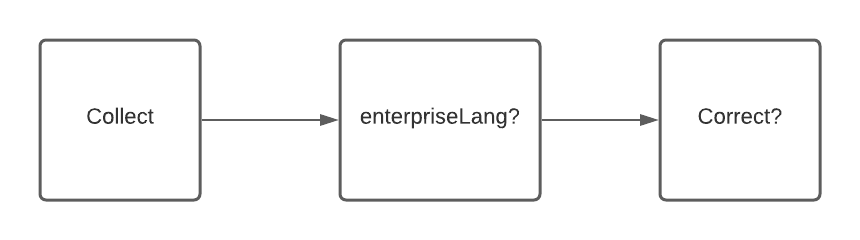
\includegraphics{researchsteps.png}
  \end{center}
  \caption{Research Process}
  \label{fig:researchsteps}
\end{figure}

\newpage
\noindent{\Large Step 1}\\

\noindent Collect real-world attacks on enterprise systems. For this step to be achieved successfully, it is important to comprehend the main concepts of threats such as security alerts, as seen in Figure~\ref{fig:researchsteps1}.

\begin{figure}[!ht]
  \begin{center}
    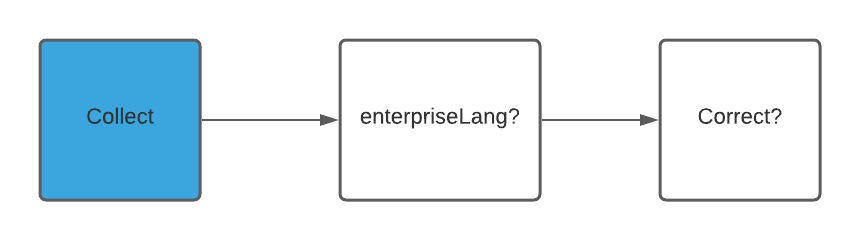
\includegraphics{researchsteps1.png}
  \end{center}
  \caption{Research Process}
  \label{fig:researchsteps1}
\end{figure}

\noindent{\Large Step 2}\\

\noindent Check whether all attack steps of each collected real-world attack are included in enterpriseLang. To accomplish this, it is crucial to understand the language enterpriseLang and its symbols, how it works and how it models an attack, as seen in Figure~\ref{fig:researchsteps2} \cite{xiong2021cyber,johnson2018mal}.

\begin{figure}[!ht]
  \begin{center}
    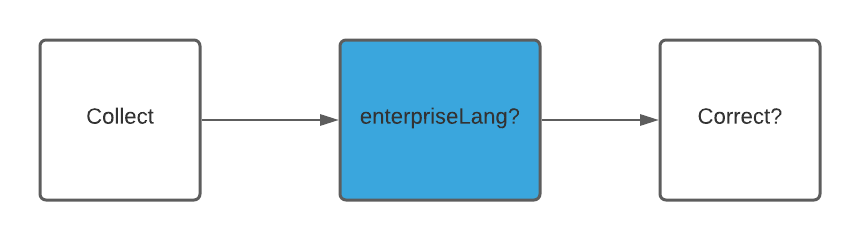
\includegraphics{researchsteps2.png}
  \end{center}
  \caption{Research Process}
  \label{fig:researchsteps2}
\end{figure}

\noindent{\Large Step 3}\\

\noindent Check if each attack path is correctly described in enterpriseLang. If not, update enterpriseLang with new attack steps and the correct attack path, as seen in Figure~\ref{fig:researchsteps3}.

\begin{figure}[!ht]
  \begin{center}
    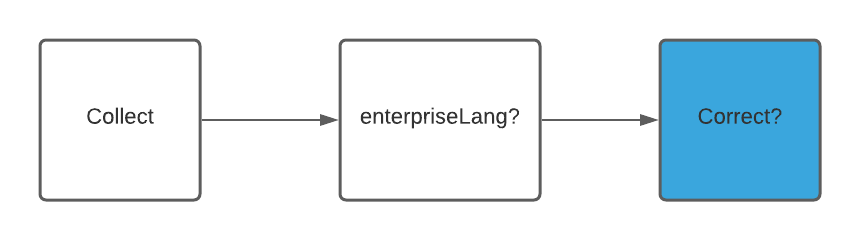
\includegraphics{researchsteps3.png}
  \end{center}
  \caption{Research Process}
  \label{fig:researchsteps3}
\end{figure}

\newpage
\section{Research Paradigm}
\label{sec:researchParadigm}
%\todo[inline, backgroundcolor=aqua]{Undersökningsparadigm}

\noindent{\Large Literature study}\\

\noindent To get the information needed for this project, literature study was chosen as a form of the research process for this work. Various paper works has been selected \cite{xiong2021cyber,johnson2018mal,hersen2021towards} that together explain the topic of this thesis which is threat modeling and attack simulations. The sources contained valuable and validated and it was reliable since all of them were a part of thesis works.\\

\noindent{\Large Design Science Research}\\

\noindent Another method used in this work was \gls{DSR}, former projects about the selected subject was used as inspirational sources and helping guidelines. Throughout the bachelor thesis, theories  deriving from the inspirational sources \cite{xiong2021cyber,johnson2018mal,hersen2021towards} were implemented.\\

\noindent{\Large Qualitative Research}\\

\noindent Qualitative research was chosen as a research method. The focus about such a research method is to gather knowledge within the subject field, to further develop information to greater extends within the topic area. Previous data from existent sources evolves into new expanded information that could be far more useful. This research method is eligible for increasing knowledge about an indefinite domain that is nearly undiscovered such as the enterpriseLang language, hence qualitative research was chosen for the bachelor thesis.

\section{Data Collection}
\label{sec:dataCollection}

\noindent The methods used for data collection was documents and observations. Documents provided by employees of MITRE ATT\&CK \cite{xiong2021cyber,johnson2018mal,hersen2021towards} were used as sample of inspiration. Databases of the same organisation, with other words databases from MITRE ATT\&CK were helpful along with the previous codes of enterpriseLang in GitHub, a platform where developers and companies build, maintain and store their software. The previous software stored in GitHub created by the earlier developers from MITRE ATT\&CK was able to be viewed and accessed to when further developing new software. The existing code could be observed neatly  to program new software from the GitHub server and it was to a big effect of assistance.

\subsection{Test environment}
\noindent There should be a test environment to check two conditions of the test cases; first condition is to check in cases the created test cases can be compiled and executed successfully. After this conditions is met it is also required in the project to validate the coverage of the test cases, this is the second condition to be met. To assess the conditions and complete both of them, it is needful to have two available software components. The first one is a Malcompiler which is a compiler suppose to build code of \gls{MAL}, in this way the student could see whether the newly created test cases could execute without errors. The second addition is \gls{MAL}-visualization, a visualization that automately visualizes solutions for \gls{MAL} based languages.

\subsection{Software to be used}
\noindent The thesis work is purely based on software, only a computer is required to evolve the project of the thesis. A code editor and a terminal, both functional enough for their purpose installed in the computer are essential parts for the thesis. Code editor is crucial for editing the software itself and a terminal such as Ubuntu which is Linux's own terminal is important for editing and saving files to saving repository, for instance GitHub which is further a vital component for the thesis to be carried on. GitHub is a platform where developers store and save software work such as projects.

\subsection{Validity and reliability}
All the data contained in the thesis is derived from MITRE ATT\&CK, the global cybersecurity company that was willing to cooperate with the author of this thesis. The validity and reliability has gone through educated beings in the enterprise. The additional papers that were favorable to the thesis is written by authors whose paper work has been validated by MITRE ATT\&CK.

\section{Ethical considerations}
\label{sec:ethicalConsiderations}
 
 With the consideration of the cooperation with an international IT company such as MITRE ATT\&CK,  there could be classified information within the organisation when researching for information being prosperous for the thesis. Both the author and the supervisor of this project confirmed and made sure that no such sensitive data would be obtained in this paper.

\clearpage
\newpage
\mbox{~}
\clearpage
\newpage
%\cleardoublepage
\chapter{Implementation}
\label{ch:implementation}

The purpose of this chapter is to describe the implementation of the thesis. Section~\ref{sec:work} describes the important parts for the work needed to be done. Section~\ref{sec:illustration} details how the implementation went on during the thesis.

\section{Work}
\label{sec:work}

\subsection{Software design}
\noindent The implementation of the project thesis was entirely based on software design. The software design was written in enterpriseLang syntaxes but it is created from the language Java. ~\url{https://GitHub.com/mal-lang/enterpriseLang} is the storage of the concluded software design so far in threat modeling and attack simulations project.

\subsection{Supplementation}
There were external additions that needed to be succeeded before being able to fully flexible in the software design. The supplements would help with testing the newly coded software design and test the limits of the programming.

\subsubsection{Malcompiler}
Malcompiler is a compiler for the \gls{MAL}, it compiles code written from the \gls{MAL} framework to validate whether a freshly coded part in a software is successfully compilable before getting to next step which is visualizing the solutions in \gls{MAL}. The link for the Malcompiler is here \url{https://GitHub.com/nicklashersen/malcompiler}.

\subsubsection{\gls{MAL}-visualization}
\gls{MAL}-visualization is an automated visualization of \gls{MAL} based software solutions. At the beginning of the project, one of the wishes was to visualize the created tests to assess the coverage of the test cases, this step couldn't be done since the \gls{MAL}-visualization took to much time and resources to get installed.

\subsubsection{Ubuntu terminal}
Another supplementation considered utterly significant was the Ubuntu terminal. When it comes to using terminals, Ubuntu is regarded as very helpful, it supports many languages and it has package manage systems which makes it easier to install and remove tools. It is also able to create, remove and change files directly when integrating with software design at the same time, it is open source meaning that you can install whatever extension without difficulties which makes it intuitive when programming with the need of a terminal. Ubuntu terminal is suitable when working in a development environment such as this thesis project.

\subsection{Storage}
GitHub was an important tool for the work to be carried on. It was used to store and save designed software. Colleague programmers could access and view code without complications and when needed, the colleagues could load the work to their computers and continue with the work. ~\url{https://GitHub.com/hassanyaasin/enterpriseLang} is the repository of the sole test codes created by the author.


\begin{comment}

Figure~\ref{fig:homepageicon} shows a simple icon for a home page. The time
to access this page when served will be quantified in a series of
experiments. The configurations that have been tested in the test bed are
listed in Table~\ref{tab:configstested}.

\begin{swedishnotes}
Figur~\ref{fig:homepageicon}  visar en enkel ikon för en hemsida. Tiden för att få tillgång till den här sidan när serveras kommer att kvantifieras i en serie experiment. De konfigurationer som har testats i provbänk listas ini tabell~\ref{tab:configstested}.

Vad du har gjort? Hur gjorde du det? Vad designen beslut gjorde du?
\end{swedishnotes}
 
\begin{figure}[!ht]
  \begin{center}
    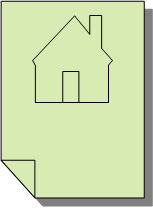
\includegraphics[width=0.25\textwidth]{Homepage-icon.png}
  \end{center}
  \caption{Homepage icon}
  \label{fig:homepageicon}
\end{figure}

\begin{table}[!ht]
  \begin{center}
    \caption{Configurations tested}
    \label{tab:configstested}
    \begin{tabular}{l|c} % <-- Alignments: 1st column left, 2nd middle and 3rd right, with vertical lines in between
      \textbf{Configuration} & \textbf{Description} \\
      \hline
      1 & Simple test with one server\\
      2 & Simple test with one server\\
    \end{tabular}
  \end{center}
\end{table}
\todo[inline, backgroundcolor=aqua]{Konfigurationer testade}
\end{comment}

\clearpage
\section{Illustration}
%\todo[inline, backgroundcolor=aqua]{Implementering … / modellering / simulering / …}
\label{sec:illustration}

\subsection{Some examples of coding}

Listing~\ref{lst:accountDiscovery} shows an example of accountDiscovery an attack written in enterpriseLang code in Java.

\begin{lstlisting}[caption={accountDiscovery attack}, label=lst:accountDiscovery]

public class TestAccountDiscovery extends EnterpriseLangTest {

    private static class accountDiscovery {
        public final UserAccount userAccount = new UserAccount("userAccount");
        public final OS os = new OS("os");
        public final Computer computer = new Computer("computer");
        
        public accountDiscovery() {
           userAccount.addOs(os);
           computer.addOs(os); 

        }
    }

    @Test
    public void userRights(){
        var model = new accountDiscovery();

        Attacker attacker = new Attacker();
        attacker.addAttackPoint(model.userAccount.userRights);
        attacker.attack();

        model.os.accountDiscovery.assertCompromisedInstantaneously();
        model.os.domainDiscovery.assertCompromisedInstantaneously();
    }

    @Test
    public void infectedOS(){
        var model = new accountDiscovery();

        Attacker attacker = new Attacker();
        attacker.addAttackPoint(model.userAccount.userRights);
        attacker.attack();

        model.os.accountDiscovery.assertCompromisedInstantaneously();
        model.os.domainDiscovery.assertCompromisedInstantaneously();
    }

    @Test
    public void domainDiscovery(){
        var model = new accountDiscovery();

        Attacker attacker = new Attacker();
        attacker.addAttackPoint(model.userAccount.userRights);
        attacker.attack();
        
        model.os.accountDiscovery.assertCompromisedInstantaneously();
        model.os.domainDiscovery.assertCompromisedInstantaneously();
    }
}
\end{lstlisting}

\noindent Listing~\ref{lst:forcedAuthentication} shows an example of a forcedAuthentication attack written in enterpriseLang code in Java.

\begin{lstlisting}[caption={forcedAuthentication attack}, label=lst:forcedAuthentication]

public class TestForcedAuthentication extends EnterpriseLangTest {
    private static class forcedAuthentication{
        public final UserAccount userAccount = new UserAccount("userAccount");
        public final OS os = new OS("os");
        public final Computer computer = new Computer("computer");

        public forcedAuthentication(){
            userAccount.addOs(os);
            computer.addOs(os);
        }
    }

    @Test
    public void userRights(){
        var model = new forcedAuthentication();

        Attacker attacker = new Attacker();
        attacker.addAttackPoint(model.userAccount.userRights);
        attacker.attack();

        model.os.forcedAuthentication.assertCompromisedInstantaneously();
    }

    @Test
    public void infectedOS(){
        var model = new forcedAuthentication();

        Attacker attacker = new Attacker();
        attacker.addAttackPoint(model.userAccount.userRights);
        attacker.attack();

        model.os.bruteForce.assertCompromisedInstantaneously();
        model.os.forcedAuthentication.assertCompromisedInstantaneously();
        model.os.domainDiscovery.assertCompromisedInstantaneously();
    }
}
\end{lstlisting}

\noindent Listing~\ref{lst:keyChain} shows an example of keyChain an attack written in enterpriseLang code in Java.

\begin{lstlisting}[caption={keyChain attack}, label=lst:keyChain]

public class TestKeyChain extends EnterpriseLangTest {

    private static class keyChain {
        public final AdminAccount adminAccount = new AdminAccount("adminAccount");
        public final UserAccount userAccount = new UserAccount("userAccount");
        public final OS os = new OS("os");
        
        public keyChain() {
            adminAccount.addOs(os);
            userAccount.addOs(os);

        }
    }

    @Test
    public void userRights(){
        var model = new keyChain();

        Attacker attacker = new Attacker();
        attacker.addAttackPoint(model.userAccount.userRights);
        attacker.attack();

        model.os.domainDiscovery.assertCompromisedInstantaneously();
        model.os.accountDiscovery.assertCompromisedInstantaneously();
    }
}

\end{lstlisting}
\subsection{Code storage}

The software code from listing ~\ref{lst:accountDiscovery}, listing~\ref{lst:forcedAuthentication} and ~\ref{lst:keyChain} originates from the GitHub repository \url{https://GitHub.com/hassanyaasin/enterpriseLang}.

\clearpage
\newpage
\mbox{~}
\clearpage
\newpage
%\cleardoublepagepage
\chapter{Results and Analysis}
\todo[inline, backgroundcolor=aqua]{svensk: Resultat och Analys}
\label{ch:resultsAndAnalysis}
\todo[inline]{
Sometimes this is split into two chapters.\\
  
Keep in mind: How you are going to evaluate what you have done? What are your metrics?\\
Analysis of your data and proposed solution\\
Does this meet the goals which you had when you started?
}

In this chapter, we present the results and discuss them.

\begin{swedishnotes}
I detta kapitel presenterar vi resultatet och diskutera dem.
\end{swedishnotes}
\todo[inline, backgroundcolor=aqua]{
Ibland delas detta upp i två kapitel.\\
Hur du ska utvärdera vad du har gjort? Vad är din statistik?\\
Analys av data och föreslagen lösning\\
Innebär detta att uppnå de mål som du hade när du började?
}

\section{Major results}
\todo[inline, backgroundcolor=aqua]{Huvudsakliga resultat}

Some statistics of the delay measurements are shown in Table~\ref{tab:delayMeasurements}.
The delay has been computed from the time the GET request is received until the response is sent.

\begin{swedishnotes}
Lite statistik av mätningarna fördröjnings visas i Tabell~\ref{tab:delayMeasurements}. Förseningen har beräknats från den tidpunkt då begäran GET tas emot fram till svaret skickas.
\end{swedishnotes}

\begin{table}[!ht]
  \begin{center}
    \caption{Delay measurement statistics}
    \label{tab:delayMeasurements}
    \begin{tabular}{l|S[table-format=4.2]|S[table-format=3.2]} % <-- Alignments: 1st column left, 2nd middle and 3rd right, with vertical lines in between
      \textbf{Configuration} & \textbf{Average delay (ns)} & \textbf{Median delay (ns)}\\
      \hline
      1 & 467.35 & 450.10\\
      2 & 1687.5 & 901.23\\
    \end{tabular}
  \end{center}
\end{table}
\todo[inline, backgroundcolor=aqua]{Fördröj mätstatistik}
\todo[inline, backgroundcolor=aqua]{Konfiguration | Genomsnittlig fördröjning (ns) | Median fördröjning (ns)}

Figure \ref{fig:processing_vs_payload_length} shows and example of the
performance as measured in the experiments.

\begin{figure}[!ht]
% GNUPLOT: LaTeX picture
\setlength{\unitlength}{0.240900pt}
\ifx\plotpoint\undefined\newsavebox{\plotpoint}\fi
\begin{picture}(1500,900)(0,0)
\sbox{\plotpoint}{\rule[-0.200pt]{0.400pt}{0.400pt}}%
\put(171.0,131.0){\rule[-0.200pt]{4.818pt}{0.400pt}}
\put(151,131){\makebox(0,0)[r]{ 1.5}}
\put(1419.0,131.0){\rule[-0.200pt]{4.818pt}{0.400pt}}
\put(171.0,212.0){\rule[-0.200pt]{4.818pt}{0.400pt}}
\put(151,212){\makebox(0,0)[r]{ 2}}
\put(1419.0,212.0){\rule[-0.200pt]{4.818pt}{0.400pt}}
\put(171.0,292.0){\rule[-0.200pt]{4.818pt}{0.400pt}}
\put(151,292){\makebox(0,0)[r]{ 2.5}}
\put(1419.0,292.0){\rule[-0.200pt]{4.818pt}{0.400pt}}
\put(171.0,373.0){\rule[-0.200pt]{4.818pt}{0.400pt}}
\put(151,373){\makebox(0,0)[r]{ 3}}
\put(1419.0,373.0){\rule[-0.200pt]{4.818pt}{0.400pt}}
\put(171.0,454.0){\rule[-0.200pt]{4.818pt}{0.400pt}}
\put(151,454){\makebox(0,0)[r]{ 3.5}}
\put(1419.0,454.0){\rule[-0.200pt]{4.818pt}{0.400pt}}
\put(171.0,534.0){\rule[-0.200pt]{4.818pt}{0.400pt}}
\put(151,534){\makebox(0,0)[r]{ 4}}
\put(1419.0,534.0){\rule[-0.200pt]{4.818pt}{0.400pt}}
\put(171.0,615.0){\rule[-0.200pt]{4.818pt}{0.400pt}}
\put(151,615){\makebox(0,0)[r]{ 4.5}}
\put(1419.0,615.0){\rule[-0.200pt]{4.818pt}{0.400pt}}
\put(171.0,695.0){\rule[-0.200pt]{4.818pt}{0.400pt}}
\put(151,695){\makebox(0,0)[r]{ 5}}
\put(1419.0,695.0){\rule[-0.200pt]{4.818pt}{0.400pt}}
\put(171.0,776.0){\rule[-0.200pt]{4.818pt}{0.400pt}}
\put(151,776){\makebox(0,0)[r]{ 5.5}}
\put(1419.0,776.0){\rule[-0.200pt]{4.818pt}{0.400pt}}
\put(171.0,131.0){\rule[-0.200pt]{0.400pt}{4.818pt}}
\put(171,90){\makebox(0,0){ 0}}
\put(171.0,756.0){\rule[-0.200pt]{0.400pt}{4.818pt}}
\put(298.0,131.0){\rule[-0.200pt]{0.400pt}{4.818pt}}
\put(298,90){\makebox(0,0){ 10}}
\put(298.0,756.0){\rule[-0.200pt]{0.400pt}{4.818pt}}
\put(425.0,131.0){\rule[-0.200pt]{0.400pt}{4.818pt}}
\put(425,90){\makebox(0,0){ 20}}
\put(425.0,756.0){\rule[-0.200pt]{0.400pt}{4.818pt}}
\put(551.0,131.0){\rule[-0.200pt]{0.400pt}{4.818pt}}
\put(551,90){\makebox(0,0){ 30}}
\put(551.0,756.0){\rule[-0.200pt]{0.400pt}{4.818pt}}
\put(678.0,131.0){\rule[-0.200pt]{0.400pt}{4.818pt}}
\put(678,90){\makebox(0,0){ 40}}
\put(678.0,756.0){\rule[-0.200pt]{0.400pt}{4.818pt}}
\put(805.0,131.0){\rule[-0.200pt]{0.400pt}{4.818pt}}
\put(805,90){\makebox(0,0){ 50}}
\put(805.0,756.0){\rule[-0.200pt]{0.400pt}{4.818pt}}
\put(932.0,131.0){\rule[-0.200pt]{0.400pt}{4.818pt}}
\put(932,90){\makebox(0,0){ 60}}
\put(932.0,756.0){\rule[-0.200pt]{0.400pt}{4.818pt}}
\put(1059.0,131.0){\rule[-0.200pt]{0.400pt}{4.818pt}}
\put(1059,90){\makebox(0,0){ 70}}
\put(1059.0,756.0){\rule[-0.200pt]{0.400pt}{4.818pt}}
\put(1185.0,131.0){\rule[-0.200pt]{0.400pt}{4.818pt}}
\put(1185,90){\makebox(0,0){ 80}}
\put(1185.0,756.0){\rule[-0.200pt]{0.400pt}{4.818pt}}
\put(1312.0,131.0){\rule[-0.200pt]{0.400pt}{4.818pt}}
\put(1312,90){\makebox(0,0){ 90}}
\put(1312.0,756.0){\rule[-0.200pt]{0.400pt}{4.818pt}}
\put(1439.0,131.0){\rule[-0.200pt]{0.400pt}{4.818pt}}
\put(1439,90){\makebox(0,0){ 100}}
\put(1439.0,756.0){\rule[-0.200pt]{0.400pt}{4.818pt}}
\put(171.0,131.0){\rule[-0.200pt]{0.400pt}{155.380pt}}
\put(171.0,131.0){\rule[-0.200pt]{305.461pt}{0.400pt}}
\put(1439.0,131.0){\rule[-0.200pt]{0.400pt}{155.380pt}}
\put(171.0,776.0){\rule[-0.200pt]{305.461pt}{0.400pt}}
\put(30,453){\rotatebox{-270}{\makebox(0,0){Processing time (ms)}}}
\put(805,29){\makebox(0,0){Payload size (bytes)}}
\put(868.0,131.0){\rule[-0.200pt]{0.400pt}{84.074pt}}
\put(995.0,131.0){\rule[-0.200pt]{0.400pt}{98.287pt}}
\put(1173.0,131.0){\rule[-0.200pt]{0.400pt}{118.041pt}}
\put(1325.0,131.0){\rule[-0.200pt]{0.400pt}{134.904pt}}
\put(1350.0,131.0){\rule[-0.200pt]{0.400pt}{137.795pt}}
\put(1439.0,131.0){\rule[-0.200pt]{0.400pt}{155.380pt}}
\end{picture}
\caption[A GNUplot figure]{Processing time vs. payload length}\vspace{0.5cm}
\label{fig:processing_vs_payload_length}
\end{figure}
		

Given these measurements, we can calculate our processing bit rate as the inverse of the time it takes to process an additional byte divided by 8 bits per byte:

\[
	bitrate = \frac{1}{\frac{time_{byte}}{8}} = 20.03 \quad kb/s
\] 

\section{Reliability Analysis}
\todo[inline, backgroundcolor=aqua]{Analys av reabilitet}
\begin{swedishnotes}
Reabilitet i metod och data 
\end{swedishnotes}

\section{Validity Analysis}
\todo[inline, backgroundcolor=aqua]{Analys av validitet}
\begin{swedishnotes}
Validitet i metod och data 
\end{swedishnotes}

\cleardoublepage
\chapter{Discussion}\todo[inline]{This can be a separate chapter or a section
  in the previous chapter.}
\todo[inline, backgroundcolor=aqua]{Diskussion}
\label{ch:discussion}
\begin{swedishnotes}
Förbättringsförslag?
\end{swedishnotes}

\cleardoublepage
\chapter{Conclusions and Future work}
\todo[inline, backgroundcolor=aqua]{Slutsats och framtida arbete}
\label{ch:conclusionsAndFutureWork}
Add text to introduce the subsections of this chapter.

\section{Conclusions}
\todo[inline]{Describe the conclusions (reflect on the whole introduction given in Chapter 1).}
\todo[inline, backgroundcolor=aqua]{Slutsatser}
\label{sec:conclusions}
  
Discuss the positive effects and the drawbacks.\\
Describe the evaluation of the results of the degree project.\\
Did you meet your goals?\\
What insights have you gained?\\
What suggestions can you give to others working in this area?\\
If you had it to do again, what would you have done differently?\\

\begin{swedishnotes}
Träffade du dina mål?
Vilka insikter har du fått?
Vilka förslag kan du ge till andra som arbetar inom detta område?
Om du hade att göra igen, vad skulle du ha gjort annorlunda?
\end{swedishnotes}

\section{Limitations}
\todo[inline]{What did you find that limited your
  efforts? What are the limitations of your results?}
\todo[inline, backgroundcolor=aqua]{Begränsande faktorer}
\label{sec:limitations}
\begin{swedishnotes}
Vad gjorde du som begränsade dina ansträngningar? Vilka är begränsningarna i dina resultat?
\end{swedishnotes}

\section{Future work}
\todo[inline]{Describe valid future work that you or someone else could or should do.\\
Consider: What you have left undone? What are the next obvious things to be done? What hints can you give to the next person who is going to follow up on your work?
}
\todo[inline, backgroundcolor=aqua]{Vad du har kvar ogjort?\\
Vad är nästa självklara saker som ska göras?\\
Vad tips kan du ge till nästa person som kommer att följa upp på ditt arbete?
}
\label{sec:futureWork}

Due to the breadth of the problem, only some of the initial goals have been
met. In these section we will focus on some of the remaining issues that
should be addressed in future work. ...

\subsection{What has been left undone?}
\label{what-has-been-left-undone}

The prototype does not address the third requirment, i.e., a yearly
unavailability of less than 3 minutes, this remains an open problem. ...

\subsubsection{Cost analysis}

The current prototype works, but the performance from a cost perspective makes
this an impractical solution. Future work must reduce the cost of this
solution, to do so a cost analysis needs to first be done. ...

\subsubsection{Security}

A future research effort is needed to address the security holes that results
from using a self-signed certificate. Page filling text mass. Page filling
text mass. ...


\subsection{Next obvious things to be done}

In particular, the author of this thesis wishes to point out xxxxxx remains as
a problem to be solved. Solving this problem is the next thing that should be
done. ...

\section{Reflections}




\noindent\rule{\textwidth}{0.4mm}
\todo[inline]{In the references, let Zotero or other tool fill this
  in for you. I suggest an extended version of the IEEE  style, to include
  URLs, DOIs, ISBNs, etc., to make it easier for your reader to find
  them. This will make life easier for your opponents and examiner. \\

  IEEE Editorial Style Manual: \url{https://www.ieee.org/content/dam/ieee-org/ieee/web/org/conferences/style_references_manual.pdf}
}
\todo[inline, backgroundcolor=aqua]{Låt Zotero eller annat verktyg fylla i det här för dig. Jag föreslår en utökad version av IEEE stil - att inkludera webbadresser, DOI, ISBN etc. - för att göra det lättare för läsaren att hitta dem. Detta kommer att göra livet lättare för dina motståndare och examinator.}

\cleardoublepage
% Print the bibliography (and make it appear in the table of contents)
%\printbibliography[heading=bibintoc]
% The lines below are for BibTeX
\bibliographystyle{myIEEEtran}
\renewcommand{\bibname}{References}
\addcontentsline{toc}{chapter}{References}
\bibliography{references}




\cleardoublepage
\appendix
\renewcommand{\chaptermark}[1]{\markboth{Appendix \thechapter\relax:\thinspace\relax#1}{}}
\chapter{Something Extra}
\todo[inline, backgroundcolor=aqua]{svensk: Extra Material som Bilaga}

\label{pg:lastPageofMainmatter}

\clearpage
\section*{For DIVA}
\divainfo{pg:lastPageofPreface}{pg:lastPageofMainmatter}
\end{document}
